\documentclass[11pt]{article}

\usepackage[a4paper]{geometry}
\geometry{left=2.0cm,right=2.0cm,top=2.5cm,bottom=2.5cm}

\usepackage{ctex} % 支持中文的LaTeX宏包
\usepackage{amsmath,amsfonts,graphicx,subfigure,amssymb,bm,amsthm,mathrsfs,mathtools,breqn} % 数学公式和符号的宏包集合
\usepackage{algorithm,algorithmicx} % 算法和伪代码的宏包
\usepackage[noend]{algpseudocode} % 算法和伪代码的宏包
\usepackage{fancyhdr} % 自定义页眉页脚的宏包
\usepackage[framemethod=TikZ]{mdframed} % 创建带边框的框架的宏包
\usepackage{fontspec} % 字体设置的宏包
\usepackage{adjustbox} % 调整盒子大小的宏包
\usepackage{fontsize} % 设置字体大小的宏包
\usepackage{tikz,xcolor} % 绘制图形和使用颜色的宏包
\usepackage{multicol} % 多栏排版的宏包
\usepackage{multirow} % 表格中合并单元格的宏包
\usepackage{pdfpages} % 插入PDF文件的宏包
\RequirePackage{listings} % 在文档中插入源代码的宏包
\RequirePackage{xcolor} % 定义和使用颜色的宏包
\usepackage{wrapfig} % 文字绕排图片的宏包
\usepackage{bigstrut,multirow,rotating} % 支持在表格中使用特殊命令的宏包
\usepackage{booktabs} % 创建美观的表格的宏包
\usepackage{circuitikz} % 绘制电路图的宏包
\usepackage{appendix}
\usepackage{listings}
\usepackage[style=numeric]{biblatex}
\usepackage{hyperref} % 引入宏包以创建可点击的链接
\hypersetup{colorlinks=true, linkcolor=blue, urlcolor=blue}


\definecolor{dkgreen}{rgb}{0,0.6,0}
\definecolor{gray}{rgb}{0.5,0.5,0.5}
\definecolor{mauve}{rgb}{0.58,0,0.82}


% 轻松引用, 可以用\cref{}指令直接引用, 自动加前缀. 
% 例: 图片label为fig:1
% \cref{fig:1} => Figure.1
% \ref{fig:1}  => 1
\usepackage[capitalize]{cleveref}
% \crefname{section}{Sec.}{Secs.}
\Crefname{section}{Section}{Sections}
\Crefname{table}{Table}{Tables}
\crefname{table}{Table.}{Tabs.}

\setmainfont{Palatino Linotype.ttf}
\setCJKmainfont{SimHei.ttf}
% \setCJKsansfont{Songti.ttf}
% \setCJKmonofont{SimSun.ttf}
\punctstyle{kaiming}
% 偏好的几个字体, 可以根据需要自行加入字体ttf文件并调用

%代码块-------------
\lstset{
  frame=tb,
  aboveskip=3mm,
  belowskip=3mm,
  showstringspaces=false,
  columns=flexible,
  framerule=1pt,
  rulecolor=\color{gray!35},
  backgroundcolor=\color{gray!5},
  basicstyle={\small\ttfamily},
  numbers=none,
  numberstyle=\tiny\color{gray},
  keywordstyle=\color{blue},
  commentstyle=\color{dkgreen},
  stringstyle=\color{mauve},
  breaklines=true,
  breakatwhitespace=true,
  tabsize=3,
}
\addbibresource{reference.bib}

\begin{document}

%若需在页眉部分加入内容, 可以在这里输入
% \pagestyle{fancy}
% \lhead{\kaishu 测试}
% \chead{}
% \rhead{}

\begin{center}
    \LARGE \bf 《利用欧拉法与荣格库塔法模拟
带电粒子在地球磁场中的运动》
\end{center}




\begin{center}
    \Large \bf 组员\qquad 冯源\, 徐盛昊\, 张天睿\, 左翔\\
    \Large \bf {\today}
\end{center}
%--------------------------
\section{背景介绍}


    \subsection{基本物理机制:洛伦兹力}
    带电粒子在电磁场中的运动遵循经典电磁学的基本规律,由洛伦兹力方程精确描述:
    \begin{equation}
        \bf{F}=q\ \cdot\ (E\ + \ \bf{v}\ \times \ \bf{B})\label{1}
    \end{equation}
    其中:
    \begin{itemize}
        \item $q$为粒子电荷量$(C)$
        \item $E$为电场强度$(V/m)$
        \item $v$ 为粒子速度$(m/s)$
        \item $B$ 为磁感应强度$(T)$
    \end{itemize}
    \subsection{地球辐射带与电子运动} 
    地球辐射带(Van Allen Belts)是环绕地球、主要由高能带电粒子(如电子和质子)组成的空间区带。1958年,Van Allen等人首次利用人造卫星观测发现了地球辐射带,这一突破揭示了地球磁场在空间环境的屏障作用。辐射带不仅在空间物理学和空间天气研究中具有基础性意义,也是当前航天技术发展中亟需关注的重要自然环境因素。高能电子对地球空间中的航天器造成潜在威胁,对电子设备、载人航天安全运营以及地球电离层环境都产生显著影响。带电粒子在地球磁场中的经典动力学可追溯到20世纪初的洛伦兹力理论,随后在Van Allen团队发现辐射带之后相关理论体系得到快速发展。Walt等学者在20世纪60年代经典著作中率先系统性提出了粒子在地球磁场中三种主要运动模式——即回旋、弹跳和漂移运动,并以此建立起环带结构与动力学之间的直接联系。粒子的回旋运动、沿磁力线的南北弹跳、以及围绕地球的缓慢漂移,正是由地球磁场的空间分布特征与洛伦兹力协同作用所导致。这一三重分解不仅为空间等离子体物理和辐射带演化机制的理解提供了理论基础,也至今仍是观测、模拟和预警高能粒子环境变化的核心动力学框架。
    \subsection{研究目标}
    本研究通过对欧拉法和荣格库塔法两种数值方法的计算精度进行对比,选定荣格库塔法作为基础,编写代码,探索粒子在地球磁场中的运动,实现绘制带电粒子在任意给定磁场中的运动轨迹的功能。本研究旨在模拟带电粒子在地球辐射带中的三种运动,验证Walt等人提出的经典物理图像。
    
%-------------------------

\section{方法引入}

根据运动学知识,可以得到表达式:
\begin{equation}
    \frac{\mathrm{d}\mathbf{r}}{\mathrm{d}t}=\mathbf{v}\label{2}
\end{equation}
\begin{equation}
    \frac{\mathrm{d}\mathbf{v}}{\mathrm{d}t}=\mathbf{a}\label{3}
\end{equation}
根据洛伦兹力表达式,可以得到表达式:
\begin{equation*}
        \bf{F}=q\ \cdot\ (E\ + \ \bf{v}\ \times \ \bf{B})
    \end{equation*}
根据牛顿第二定律,可以得到表达式:
\begin{equation}
    \mathbf{F}=m\ \cdot\ \bf{a}\label{4}
\end{equation}
将\cref{1} \cref{2} \cref{3} 式带入\cref{4}式,可以得到:
\begin{equation}
    q\ \cdot \ (E+\bf{v}\ \times \ \bf{B})=m\ \cdot\ \frac{\mathrm{d}\bf{v}}{\mathrm{d}t}\label{5}
\end{equation}
整理得到:
\begin{equation}
    \frac{\mathrm{d}\bf{v}}{\mathrm{d}t}=\frac{q}{m}\ \cdot \ (E+\bf{v}\ \times \ \bf{B}) \label{6}
\end{equation}
考虑实际情况,带电粒子在地磁场中运动速度大,动能高,$\bf{v}\ \times \bf{B}$这一项对于粒子运动占主导地位,为后续运算方便,节约算力,可忽略$E$,仅考虑$\bf{v}\ \times \bf{B}$对粒子运动带来的影响。



在三维环境中,$\bf{v}\ \times \bf{B}$ 可以在$x,y,z$三个方向展开,因而可以分方向将\cref{6}式展开得到:
\[
\frac{\mathrm{d}\mathbf{r}_x}{\mathrm{d}t} = \mathbf{v}_x
\]

\[
\frac{\mathrm{d}\mathbf{v}_x}{\mathrm{d}t} = \frac{q}{m} \cdot (\mathbf{v}_x \times \mathbf{B})
\]

\[
\frac{\mathrm{d}\mathbf{r}_y}{\mathrm{d}t} = \mathbf{v}_y
\]

\[
\frac{\mathrm{d}\mathbf{v}_y}{\mathrm{d}t} = \frac{q}{m} \cdot (\mathbf{v}_y \times \mathbf{B})
\]

\[
\frac{\mathrm{d}\mathbf{r}_z}{\mathrm{d}t} = \mathbf{v}_z
\]

\[
\frac{\mathrm{d}\mathbf{v}_z}{\mathrm{d}t} = \frac{q}{m} \cdot (\mathbf{v}_z \times \mathbf{B})
\]


求解带电粒子在磁场中的运动轨迹,本质上是在求解上述常微分方程。只要给定初值($r_0,t_0$),即可通过迭代求解下一时刻粒子的位置。利用欧拉法和荣格库塔法,可以绘制出不同时刻粒子所在的位置,进而求得粒子运动轨迹。
%-----------------------------
\section{欧拉法与荣格库塔法}
常微分方程(ODE)数值解法是解决动力学系统的核心工具,其本质是将连续时间问题离散化为迭代计算问题。对于初值问题:
\begin{equation*}
    \frac{\mathrm{d}y}{\mathrm{d}t}=f(x,y)
\end{equation*}
\begin{equation*}
    y(t_0)=y_0
\end{equation*}
欧拉法和龙格-库塔法通过不同精度的离散逼近获得数值解。


欧拉法是最简单的显式单步法,基于一阶泰勒展开:

$$y_{n+1}=y_n+f(t_n,y_n)\ \cdot\ h$$

其中h是时间步长。


龙格-库塔法通过多阶段斜率加权平均提高精度,使用四阶荣格库塔法,其通用形式:\\
$$
\begin{gathered}
y_{n+1}=y_n+\frac{h}{2}\left(k_1+2 k_2+2 k_3+k_4\right) \\
k_1=f\left(t_n, y_n\right) \\
k_2=f\left(t_n+\frac{1}{2} h, y_n+\frac{1}{2} h k_1\right) \\
k_3=f\left(t_n+\frac{1}{2} h, y_n+\frac{1}{2} h k_2\right) \\
k_4=f\left(t_n+h, y_n+h k_3\right)
\end{gathered}
$$
%----------------------------------
\section{欧拉法与改进欧拉法模拟带电粒子在匀强磁场中的运动}
数值方法的选择直接影响计算精度与效率。欧拉法(Euler method)作为最基础的一阶显式迭代算法,因其原理简单、计算量小而被广泛应用,但存在精度较低、误差积累显著的缺点。改进欧拉法(又称 Heun 方法)通过引入预测 - 校正机制,将算法精度提升至二阶,有效降低了误差增长速率。


以匀强磁场中带电粒子的三维运动为对象,对比欧拉法与改进欧拉法的数值模拟效果。通过理论推导两种方法的局部截断误差与全局误差,结合具体算例分析步长对误差的影响规律,并利用 Python 代码实现算法逻辑与可视化。

\subsection{欧拉法}
对于初值问题:
\begin{equation*}
    \frac{\mathrm{d}y}{\mathrm{d}x}=f\left(x,y\right),\ \ \  y\left(x_0\right)=y_0
\end{equation*}
而欧拉法的迭代公式:
\begin{equation*}
y_{\left(n+1\right)}=y_n+hf\left(x_n,y_n\right)\mbox{(其中,h 是步长)}
\end{equation*}
运用到匀强磁场中,对v与r迭代,即可画出粒子的运动轨迹,同时用
\begin{equation*}
\begin{gathered}
    x\left(t\right)=v_y0/k-v_y0/kcos{\left(kt\right)}+v_x0/ksin{\left(kt\right)}\\
    y(t)=-v_{x0}/k+v_{x0}/kcos{(kt)}+v_{y0}/ksin{(kt)}\\
    y(t)=-v_{x0}/k+v_{x0}/kcos{(kt)}+v_{y0}/ksin{(kt)}\\
    z\left(t\right)=v_{z0}\cdot t
\end{gathered}
\end{equation*}
模拟解析解,可以得到下图(其中$k=\frac{q\ B}{m}$):
\newpage

\begin{figure}[h!]
    \centering
    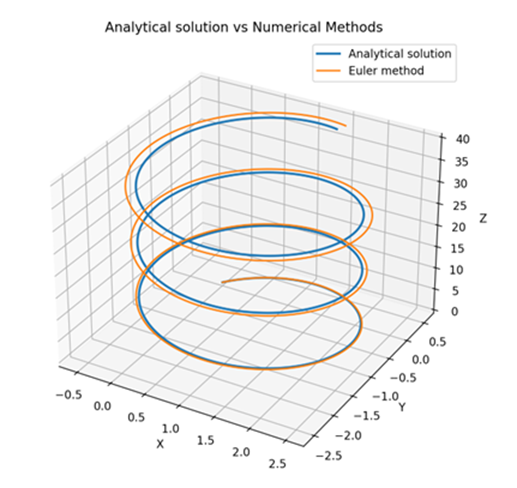
\includegraphics[width=0.5\linewidth]{Fig/Euler Method.png}
    \caption{欧拉法中解析解与数值解的比较}
    \label{fig:1}
\end{figure}


\subsection{改进欧拉法}
改进欧拉法公式为:
\begin{equation*}
    y^*=y_n+hf(x,y)
\end{equation*}

\begin{equation*}
    y_{(n+1)}=y_n+\frac{h}{2}[f(x,y)+f(x_{n+1},y^*)]
\end{equation*}

与解析解和欧拉法作对比
\begin{figure}[h!]
    \centering
    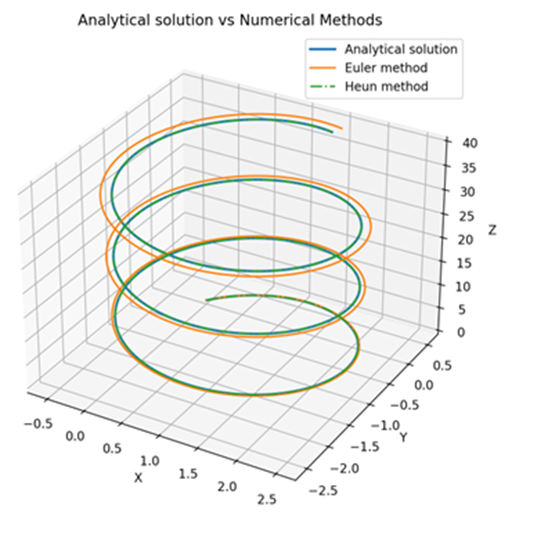
\includegraphics[width=0.5\linewidth]{Fig/Heun Method.png}
    \caption{欧拉法、改进欧拉法数值解与解析解对比}
    \label{fig:2}
\end{figure}

\subsection{误差分析}
对于局部截断误差和全局误差,其计算公式如下
\begin{equation*}
    \tau_{\left(n+1\right)}=y\left(x_{\left(n+1\right)}\right)-y\left(x_n\right)-hf\left(x_n,y\left(x_n\right)\right)=O\left(h^2\right)
\end{equation*}

\begin{equation*}
    e_n=y\left(x_n\right)-y_n
\end{equation*}
对欧拉法的真实解泰勒展开
\begin{equation*}
    \left(x\left(n+1\right)\right)=y\left(x_n\right)+hy^\prime\left(x_n\right)+h^2/2y^{\prime\prime}\left(\xi_n\right)
\end{equation*}
带入公式可得到欧拉法的局部截断误差
\begin{equation*}
    \tau\left(n+1\right)=y\left(x_{\left(n+1\right)}\right)-y\left(n+1\right)=h^2/2y^{\prime\prime}\left(\xi_n\right)
\end{equation*}
可以得到理论局部截断误差$O(h^2)$, 全局误差$O(h)$,对于改进欧拉法在n点作泰勒展开
\begin{equation*}
    y\left(x_{\left(n+1\right)}\right)=y\left(x_n\right)+hy^\prime\left(x_n\right)+h^2/2y^{\prime\prime}\left(x_n\right)+O\left(h^3\right)
\end{equation*}
而 $$y'(x_n)=f(x_n,y^*)=f(x_n+h,y(x_n)+hf(x_{(n+1)},y^*)$$也做泰勒展开:
\begin{equation*}
    f\left(x_{\left(n+1\right)},y^\ast\right)=f\left(x_n+h,y\left(x_n\right)+hf\left(x_n,y\left(x_n\right)\right)\right)+O\left(e^\ast\right)
\end{equation*}

\begin{equation*}
    \left(x_{n+1},y^\ast\right)=f\left(x_n,y\left(x_n\right)\right)+hf_x\left(x_n,y\left(x_n\right)\right)+hf_y\left(x_n,y\left(x_n\right)\right)f\left(x_n,y\left(x_n\right)\right)+O\left(h^2\right)
\end{equation*}
带入公式:
\begin{equation*}
    \begin{gathered}    y_{\left(n+1\right)}=y\left(x_n\right)+h/2\left[f\left(x_n,y\left(x_n\right)\right)+f\left(x_{\left(n+1\right)},y^\ast\right)\right]\\
    =y(x_n\ )+h/2\ {2f(x_n,y(x_n\ ))+hf_x\ (x_n,y(x_n\ )+hf_y\ (x_n,y(x_n\ ))f(x_n,y(x_n\ ))}+O(h^3\ )\\
    =y\left(x_n\right)+hf\left(x_n,y\left(x_n\right)\right)+h^2/2\left[f_x\left(x_n,y\left(x_n\right)\right)+f_y\left(x_n,y\left(x_n\right)\right)f\left(x_n,y\left(x_n\right)\right)\right]+O\left(h^3\right)
    \end{gathered}
\end{equation*}
可得局部误差$\tau_{\left(n+1\right)}=O\left(h^3\right)$,全局误差为$O\left(h^2\right)$


而在数值计算中的到的误差域步长关系如下,与理论符合:

\begin{table}[h]
    \centering
    \begin{tabular}{|c|c|c|}
        \hline
        步长 dt & 欧拉法误差 & 改进欧拉法误差\\ \hline
         0.1& 2.415891 & 0.043878\\ \hline
         0.05& 0.916474 & 0.010980\\ \hline
         0.025& 0.401586 & 0.002747\\ \hline
    \end{tabular}
    \caption{各方法误差域步长关系}
    \label{tab:my_label1}
\end{table}
其中误差通过计算最后一个点的欧几里得距离获得

%----------------------------------
\section{龙格-库塔法模拟带电粒子在匀强磁场中的运动}
\subsection{数值模拟}
    使用欧拉法和改进欧拉法之后,我们再使用龙格-库塔法来对匀强磁场中带电粒子进行分析,对于初值问题:
    \begin{equation*}
        \frac{\mathrm{d}y}{\mathrm{d}x}=f(x,y),\ \ y(x_0)=y_0
    \end{equation*}
    龙格-库塔方法的迭代公式为:
    
    \begin{equation*}
        \begin{gathered}
            y_{n+1}=y_n+\frac{h}{2}\left(k_1+2 k_2+2 k_3+k_4\right) \\
            k_1=f\left(t_n, y_n\right) \\
            k_2=f\left(t_n+\frac{1}{2} h, y_n+\frac{1}{2} h k_1\right) \\
            k_3=f\left(t_n+\frac{1}{2} h, y_n+\frac{1}{2} h k_2\right) \\
            k_4=f\left(t_n+h, y_n+h k_3\right)
        \end{gathered}
    \end{equation*}
我们有两个常微分方程为:\cref{2}和\cref{3}.


计算出解析解,并通过模拟我们可以得到以下的数值解与解析解的对比图:
\begin{figure}[h]
    \centering
    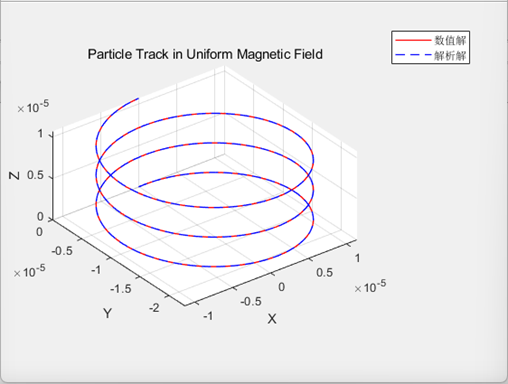
\includegraphics[width=0.5\linewidth]{Fig/RK.png}
    \caption{龙格库塔法解析解与数值解对比}
    \label{fig:3}
\end{figure}
\newline
\subsection{误差分析}
四阶龙格库塔局部阶段误差于步长的5次方成正比,我们接下来将RK4数值解进行泰勒展开(假设 f 是光滑函数,所有导数存在)。
\begin{equation*}
    \begin{gathered}
        y(t_{n+1})=y(t_n)+hy'(t_n)+\frac{h^2}{2!}y''(t_n)+\frac{h^3}{3!}y'''(t_n)+\frac{h^4}{4!}y^{(4)}(t_n)+O(h^5).\\
        \mbox{由于}y'=f(t,y),\mbox{高阶导数可以用}f\mbox{的偏导数表示:}\\
        y'(t_n)=f_n\\
y''(t_n)\frac{df}{dt}=f_t+f_yf\\
y'''(t_n)=\frac{d^2f}{dt^2}=f_{tt}+2f_{ty}f^2+f_tf_y+f_yf_t+f_y^2f=f_{tt}+2f_{ty}f+f_{yy}f^2+2f_tf_y+f^2_yf\\
y^{(4)}=...\\
\mbox{将RK4的}k_1\mbox{到}k_4\mbox{在}(t_n,y_n)\mbox{处展开,并带入}y_{n+1}\mbox{的表达式,展开到}h^4\mbox{项,有:}\\
k_1=f_n\\
k_2=f_n+\frac{1}{2}(f_t+ff_y)+\frac{h^2}{8}(f_{tt}+2ff_{ty}+f^2f_{yy}+\frac{h^3}{48}(f_{ttt}+...)+H(h^4))\\
k_3=...\\
k_4=...\\
\mbox{结果为:}y(t_{n+1})=y(t_n)+hf_n+\frac{h^2}{2}(f_t+ff_y)+\frac{h^3}{6}(f_{tt}+2f_{ty}f+f_{yy}f^2+f^2_yf)+\frac{h^4}{24}y^{(4)}+O(h^5)\\
\mbox{因此差值}\delta_{n+1}=y(t_{n+1})-y_{n+1}=O(h^5)\\
\mbox{所以我们得到了龙格库塔法的局部误差为}O(h^5)\\
\mbox{全局误差}e_n=|y_n-y(t_n)|\mbox{是积累误差,设积分区间为}[a,b],\mbox{步长为}h,\mbox{步数为}\frac{b-1}{n}\\
\to e_{n+1}\leq(1+Lh)e_n+|\delta_{n+1}|\\
\mbox{其中局部误差有}|\delta_{n+1}|\leq Kh^5\mbox{(其中}K\mbox{是常数,依赖于} f \mbox{的导数和区间长度)}\\
e_{n+1}\leq(1+Lh)e_n+Kh^5,\mbox{迭代从}e_0=0\mbox{开始}\\
e_n\leq Kh^5\sum^{n-1}_{k=0}(1+Lh)^k\\
    \end{gathered}
\end{equation*}
\begin{equation*}
    \begin{gathered}
    \mbox{几何级数为}\sum^{n-1}_{k=0}(1+Lh)^k=\frac{(1+Lh)^n-1}{Lh}\\
        \mbox{由于}nh\leq b-1,\mbox{且}(1+Lh)^n\leq e^{Lnh}\leq e^{L(b-a)},\mbox{因此}\\
e_n\leq Kh^5\cdot \frac{e^{L(b-a)}-1}{Lh}=\frac{K(e^{L(b-a)}-1)}{L}h^4\\
\mbox{即}e_n\leq Ch^4\\
\mbox{所以龙格库塔法的全局误差与}h^4\mbox{成正比,即}O(h^4)
    \end{gathered}
\end{equation*}
将步长减小看每一步的误差可以得到以下表格:

\begin{table}[h]
    \centering
    \begin{tabular}{|c|c|c|} \hline
        步长 dt &最大绝对误差  & 平均绝对误差\\ \hline
         5$\cdot 10^{-4}$& $2.757\cdot 10^{-7}$ & $1.381\cdot 10^{-7}$\\ \hline
         5$\cdot 10^{-5}$& $2.757\cdot 10^{-11}$ & $1.381\cdot 10^{-11}$\\ \hline
         5$\cdot 10^{-6}$& $2.757\cdot 10^{-15}$ & $1.381\cdot 10^{-15}$\\ \hline
    \end{tabular}
    \caption{RK方法步长与误差关系}
    \label{tab:my_label2}
\end{table}
每当步长减少为上一个步长的$\frac{1}{10}$,误差减小为原误差的$\frac{1}{10^4}$,与理论符合.
%-------------------
\section{利用荣格库塔法模拟带电粒子在均匀偶极磁场的运动轨迹}
\subsection{偶极磁场在直角坐标系下的展开}
地球的磁偶极子磁场在以地心为原点的直角坐标系 (x,y,z) 中(通常设 z 轴指向地理北极,磁偶极矩\ $M_{d\ }$沿\ z\ 轴),其磁感应强\ B\ 的三个分量($B_x,B_y{\ B}_z$) 可以表示为位置矢量\ $r=(x,y,z)的函数$。直角坐标系下磁场计算公式如下:
\begin{equation*}
    \begin{gathered}
        B_x=\frac{3μ_0M_d}{4πr^5}xz\\
        B_y=\frac{3μ_0M_d}{4πr^5}yz\\
        {\ B}_z=\frac{\mu_0M_d}{4\pi r^5}(3z^2-r^2)
    \end{gathered}
\end{equation*}



其中,$B_x, B_y, {\ B}_z$ 代表磁感应强度 $B$ 在 $x,y,z$ 三个方向上的分量。$\mu_0$代表真空磁导率,$M_d$代表地球磁偶极矩的大小。$r$ 代表粒子到地心的距离,其计算公式为$r=\sqrt{x^2+y^2+z^2}$。$x,y,z$代表粒子在直角坐标系中的三个坐标分量。

\subsection{参数设置}
粒子电荷 $q=1.602\times10^{-19}C$,粒子质量 $m=1.6726\times10^{-27kg}$,地球磁偶极矩$M_d=7.94\times10^{22}A⋅m^2$,粒子初始动能 $E_k=20k\ eV$。初始位置 $r_0=(5R_E\frac{\sqrt{2}}{2},5R_E\frac{\sqrt{2}}{2},0)$,其中$R_E=6.371\times{10}^6m$为地球半径。这意味着粒子初始位于赤道面内,距离地心约$5R_E$的地方。初始速度$\ \mathbf{v}_{0\ }$的大小由动能决定,方向为 $(\cos{(\frac{\pi}{4})},\cos{(\frac{\pi}{3})},\sin{(\frac{\pi}{3}))}) $的归一化方向乘以速度大小。时间步长 $\mathrm{d}t=5\times 10^{-4}s$,总模拟时间 $T=6\times{10}^4s$。


\clearpage

\subsection{数值模拟结果与分析}
由于质子的速度很大,因忽略电场对粒子的影响,只考虑偶极磁场对粒子的影响。通过1亿两千万次的迭代,我们成功模拟出20keV的电子在偶极磁场的运动轨轨迹。图4展示了带电粒子在地球磁场的全局运动轨迹。其中,可明显看出粒子南北向的弹跳运动和东西向的漂移运动。

\begin{figure}[h]
    \centering
    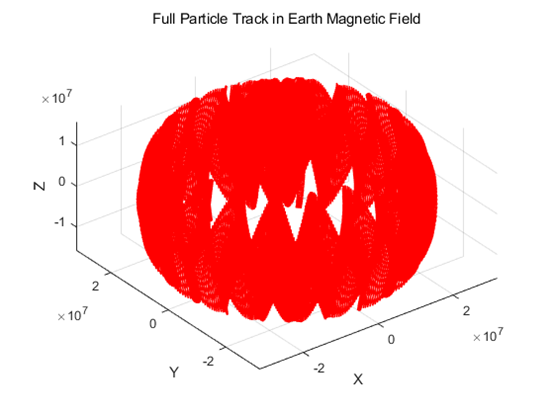
\includegraphics[width=0.75\linewidth]{Fig/fulltrack.png}
    \caption{带电粒子在地球磁场的全局运动轨迹}
    \label{fig:4}
\end{figure}


为了进一步分析带电粒子的回旋运动,我们截取了全局运动轨迹中一部分轨迹进行放大,得到了粒子的局部运动图像(图5)。根据Walt等学者给出的经验公式,回旋运动的时间尺度约在${10}^{-4}$次方秒量级。而弹跳运动和漂移运动的时间分别在秒量级和分钟量级。由图5的局部放大可以看出,粒子在南北弹跳的同时,也在做沿着磁力线的回旋运动,这与经典的物理图像相一致。

\begin{figure}[h]
    \centering
    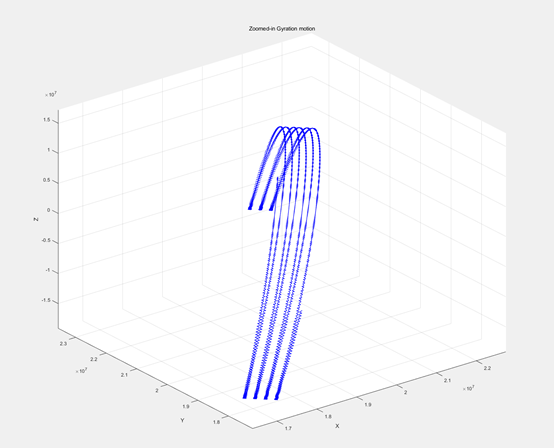
\includegraphics[width=0.5\linewidth]{Fig/zoompart.png}
    \caption{带电粒子的回旋运动(局部放大)}
    \label{fig:5}
\end{figure}



此外,\cref{fig:6}展示了\cref{fig:4}在直角坐标系的三个平面下的投影。\cref{fig:6}中左图清晰展示了带电粒子东西向的漂移运动,这与Walt等学者在20世纪60年代得出的结论一致。Walt等学者认为,由于磁场在径向上存在梯度,粒子运动的回旋半径在一个回旋周期内会发生改变。从宏观上看,这导致了电子东西向的漂移运动。\cref{fig:6}中另外两图清晰展示了带电粒子南北向的弹跳运动,这也与Walt等学者在20世纪60年代得出的结论一致。Walt等学者认为,在不受电磁波的干扰下,带电粒子的磁矩(也称第一绝热不变量)需守恒。当粒子从低纬地区运动到高纬地区,其所在位置的磁场增强。为了使得磁矩守恒,带电粒子的投掷角要增大。投掷角表示带电粒子沿磁力线运动方向和实际运动方向的夹角。在某一时刻,带电粒子的投掷角将增大到90度,即到达“磁镜”点。粒子在此处发生反射,向反方向运动。

\begin{figure}[h]
    \centering
    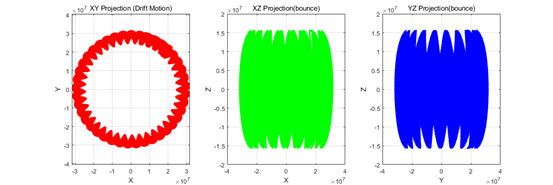
\includegraphics[width=0.75\linewidth]{Fig/projection_2.png}
    \caption{带点粒子的轨迹在三分量上的投影}
    \label{fig:6}
\end{figure}

%--------------------
\section{总结与展望}
本研究首先对比分析了欧拉法与四阶龙格-库塔(RK4)法在求解带电粒子运动常微分方程组时的数值特性。结果表明,RK4方法凭借其高阶精度,在模拟粒子轨迹时展现出更小的累积误差和更高的稳定性,是模拟带电粒子在复杂电磁场中长期运动的更优选择。基于此,我们采用RK4方法对20keV质子在理想地球偶极磁场中的运动轨迹进行了数值模拟。模拟结果成功再现了带电粒子在地球磁场中被俘获后典型的三种准周期运动模式:快速的绕磁力线的回旋运动、沿磁力线在南北半球磁镜点之间的弹跳运动、以及缓慢的环绕地球的梯度曲率漂移运动。通过对这三种运动成因的分析,本模拟结果与Walt等人在20世纪60年代对俘获粒子运动的基本物理图像描述相一致,验证了所用数值方法的有效性和对基本物理过程的准确再现能力。


尽管本研究成功模拟了带电粒子在简化地球偶极磁场中的基本运动,但其仍有广阔的拓展和深化空间。首先,当前模型仅考虑了地球磁场的零阶偶极项。真实的地球磁场更为复杂,包含了高阶多极矩项,且地磁轴与地球自转轴存在约11°的夹角。 未来的工作可以通过修改 get\_electromagneticfield 函数,引入更精确的国际地磁参考场模型(IGRF)或Tsyganenko模型等,以模拟粒子在更逼真地球磁场中的行为,这将更准确地反映粒子在真实近地空间环境中的复杂轨迹和分布。


其次,地球磁场并非静态,它受到太阳风的持续扰动以及日冕物质抛射(CME)等剧烈太阳活动的显著影响,表现出日变化、磁暴期增强等时变特性。 若能获取这些磁场变化的解析表达式或经验模型,便可将时间依赖的磁场引入模拟,从而追踪带电粒子在更大时间尺度上的动态演化,这对于理解空间天气事件中辐射带粒子的加速和损失机制至关重要。


再者,本研究聚焦于粒子在相对“平滑”的背景大尺度磁场中的运动。实际上,测试粒子模拟的思想也被广泛应用于研究带电粒子在等离子体波动(如哨声波、电磁离子回旋波等)中的相互作用。 虽然存在如福克-普朗克型扩散方程等理论模型描述粒子在波动中的一般扩散行为,但这些方程在强湍流或特定波模条件下存在局限性。通过测试粒子模拟,可以直接追踪粒子在具体波场中的精确相位和能量变化,其结果可与理论模型及卫星观测数据进行对比验证,为理解波粒相互作用的微观物理过程提供有力工具。
\clearpage

此外,本研究仅模拟了单个测试粒子的运动。在实际的空间物理研究中,如Liu等人(2012)的工作所示,通常需要同时模拟成千上万个具有特定初始分布(如能量谱、投掷角分布)的测试粒子, 通过统计分析它们的整体行为来推断宏观的粒子通量变化、相空间密度演化等。这种多粒子模拟能够更全面地反映粒子群的集体效应和统计特性。


综上所述,尽管本研究的起点是单个粒子在理想磁场中的运动这一经典问题,但其核心的测试粒子模拟方法——以龙格-库塔法等高精度数值积分为基础——仍然是当前空间物理、等离子体物理等前沿领域不可或缺的研究手段。 通过调整输入参数,如粒子初始条件、背景场模型(电磁场、波动场)、甚至引入粒子间的相互作用,该方法能够灵活地应用于探索多样化和复杂环境下的粒子动力学问题。这正是本研究工作的意义所在,也为未来的深入探索指明了方向。

\nocite{*}
\clearpage
\printbibliography

%--------------------
\clearpage
\begin{center}
    \huge\textbf{附录}
\end{center}
\vspace{1em} 

\appendix
\section{源代码}

本文的全部源代码及相关资源见 GitHub 

\begin{itemize}
    \item \textbf{GitHub 仓库地址:} \href{https://github.com/coldfish789/ESS205projectCode}{https://github.com/coldfish789/ESS205projectCode}

\end{itemize}

\end{document}